\section{Backend}
Vybral jsem si Supabase jako řešení backendu pro svůj projekt, protože nabízí open-source alternativu k Firebase s výkonnou PostgreSQL databází, která umožňuje flexibilní práci s daty, dále nabízí i bezplatný tier služby pro vývoj. Díky vestavěné podpoře pro autentizaci, realtime synchronizaci a serverless funkce poskytuje moderní a škálovatelné řešení bez nutnosti správy složité infrastruktury. Díky modulům se Supabase dobře integruje s Nuxt 3 a usnadňuje vývoj díky přehlednému API a skvělé dokumentaci.\cite{NuxtSupabase, supabasedocs}
\subsection{Ověření uživatele}
Supabase využívá tabulku \textit{auth.users} pro ověřování uživatelů, kterou spravuje automaticky. Když se někdo zaregistruje pomocí e-mailu a hesla, jeho účet se uloží do této tabulky. Zároveň mu systém automaticky odešle e-mail s potvrzovacím odkazem, který je nutné kliknutím ověřit, aby byl účet aktivován.\cite{supabseAuth, JohnKomarnicki}
\newline
Kromě toho Supabase podporuje i další metody autentizace, jako je přihlášení přes externí poskytovatele (např. Google, GitHub) nebo přihlášení pomocí magic linku, přičemž Supabase zajišťuje bezpečnost a šifrování citlivých údajů.\cite{supabseAuth} Bohužel kvůli zbytečné složitosti ze strany Googlu při přidání Google authenticatoru jsem se rozhodl zůstat pouze u e-mailu a klasického hesla.
\subsection{Middleware}
Middleware je software nebo kód, který funguje jako prostředník mezi různými částmi aplikace, například mezi klientem a serverem nebo mezi různými vrstvami v aplikaci. Obvykle se používá k manipulaci s požadavky a odpověďmi, autentizaci, logování, zpracování chyb nebo modifikaci dat předtím, než se dostanou k hlavní aplikaci. \cite{geeksforgeeks-2024}
\newline
V mém projektu slouží middleware k tomu, abych ověřil, zda je uživatel přihlášený, když se snaží dostat na části webové stránky, kde je to nutné; například na uživatelský profil.\cite{LearnVue}. Na ukázce \ref{middleware} je možné vidět jednoduchý kód, který ověří, zdali je uživatel přihlášen, a pokud není, přesměruje ho na login page.

\begin{lstlisting}[style=JavaScript, firstnumber = 1, caption={middleware/auth.js, middleware}, label={middleware}]
export default defineNuxtRouteMiddleware(() => {
    const user = useSupabaseUser();
    if (!user.value) {
        return navigateTo('/login');
    }
});}
\end{lstlisting}
Middleware pak jde snadno použít na libovolné stránce. Jeho názorné použití lze najít na ukázce \ref{middleware2}
\begin{lstlisting}[style=JavaScript, firstnumber = 2, caption={pages/profile.vue, ověření přihlášeného uživatele}, label={middleware2}]
definePageMeta({
    middleware: ["auth"],
});
\end{lstlisting}
\subsection{Struktura databáze}
Data jsou ukládána do 4 tabulek viz obrázek \ref{fig:scheme}. Tyto tabulky jsou propojené přes \textit{graph id}. Tedy každý node, edge a layout spadá pod nějaký graf.

\begin{figure}[h]
    \centering
    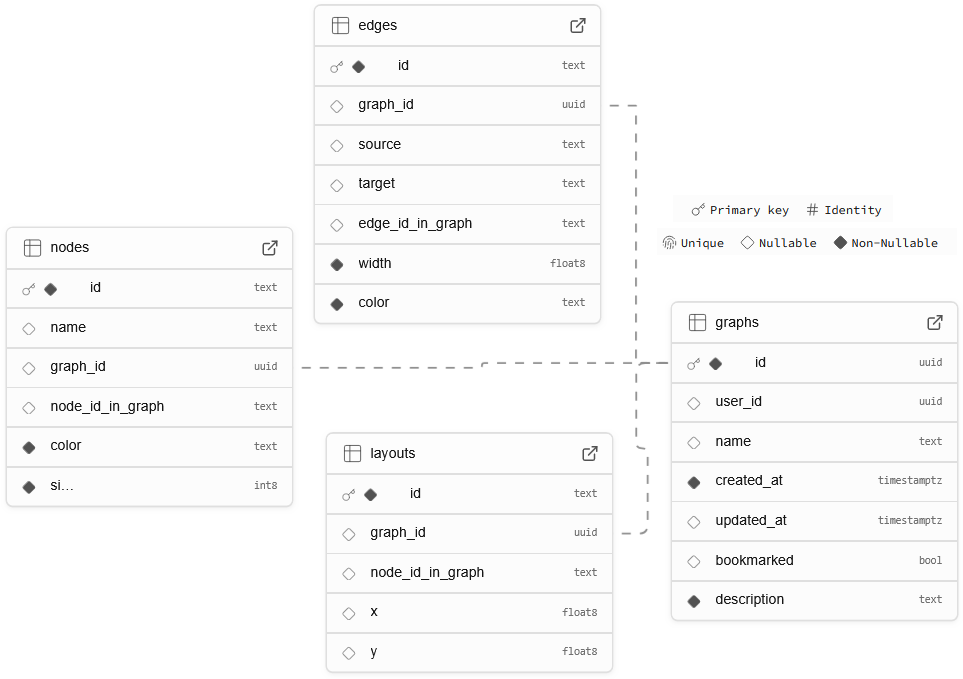
\includegraphics[width=1.1\linewidth]{Images/scheme.png}
    \caption{Schéma databáze}
    \label{fig:scheme}
\end{figure}
Za zmínku také stojí, že kvůli jednodušší implementaci s knihovnou v-network-graph, jsem se rozhodl pro propojení jednotlivých prvků grafu přes \textit{id in graph} a nikoliv propojení samotných tabulek pomocí cizího klíče. Jelikož každý node je ve v-network-graph grafové struktuře používán jako klíč, tak někdy i jako hodnota objektu viz ukázka \ref{mapping}. Tohle mé řešení sice není konvenční, nicméně mi to ulehčilo práci při mapování získaných dat z databáze.
\begin{lstlisting}[style=JavaScript, firstnumber = 1, caption={Demonstrace problému s mapováním}, label={mapping}]
// Ukazkova data
const nodes: Nodes = {
  node1: { name: "Rocket", color: "#2c3e50", size: 100 },
  node2: { name: "Fuel",color: "#2ecc71", size: 50  },
}
const edges: Edges = {
  edge1: { source: "node1", target: "node2", color: "#2c3e50", width: 8 },
}

\end{lstlisting}
\subsection{Dotazy do databáze}
Dotazy do databáze zařizují soubory \textit{graphService.js} a \textit{graphMetadataService.js}. Soubor \textit{graphService} se stará přímo o data konkrétního grafu. Kdežto \textit{graphMetadataService} se stará o metadata jednotlivých grafů, tedy posílá dotazy na jméno myšlenkové mapy, poslední datum editace a podobné.
\newline
Na ukázce \ref{dbrequest} je k nalezení část funkce \textit{fetchData}. Tato ukázka slouží jako demonstrace jednoduchého dotazu do databáze. Jako argument potřebuje objekt \textit{useSupabaseClient()} a id grafu, jehož data chceme dotazem získat.\cite{NetNinja1}

\begin{lstlisting}[style=JavaScript, firstnumber = 206, caption={utils/graphService.js, dotaz do databáze}, label={dbrequest}]
async function fetchData(supabase, graph_id) {
  const { data: nodesData, error: nodesError } = await supabase
    .from('nodes')
    .select('*')
    .eq('graph_id', graph_id);
  if (nodesError) throw nodesError;
}
\end{lstlisting}
\subsection{Row-level security}
RLS (Row-Level Security) jsou v Supabase bezpečnostní pravidla, která určují, kdo může přistupovat k jednotlivým řádkům tabulky v databázi. Supabase používá PostgreSQL Row-Level Security (RLS) k omezení přístupu na základě definovaných podmínek.\cite{RLC}
\newline
Na obrázku \ref{fig:RLC} je možné vidět RLC pro tabulku \textit{graphs} . Tato podmínka je vyhodnocována vždy při dotazu a danou akci databáze provede pouze, jestliže je pravidlo splněno. V tomto konkrétním případě může smazat user jenom svůj vlastní graf.
\begin{figure}[h]
    \centering
    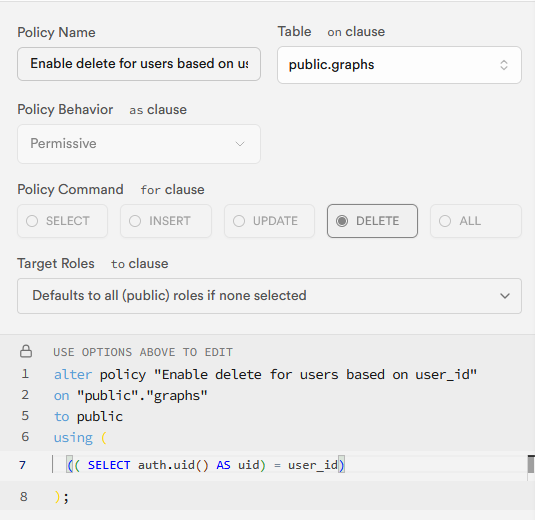
\includegraphics[width=0.6\linewidth]{Images/RLC.png}
    \caption{Příklad Supabase RLC}
    \label{fig:RLC}
\end{figure}
\subsection{Ukládání změn v grafu}
Na ukázce \ref{savegraph} je popsána funkce, která kompletně řeší problematiku uložení dat grafu. Nejprve pošle dotaz do databáze na získání všech ID pro daný graf. Následně vyfiltruje pouze ta ID, která jsou uložena v databázi, ale už ne lokálně v prohlížeči \cite{W3}; uživatel je tedy smazal. Pošle delete dotaz do databáze na tato vybraná data. Následně upsertne všechna data, která graf v prohlížeči obsahuje. Nová data jsou tedy přidána a změněná jsou updatnuta. Jde o jednoduché v celku elegantní řešení, které je konzistentní a spolehlivé.
\begin{lstlisting}[style=JavaScript, firstnumber = 168, caption={utils/graphService.js, uložení grafu}, label={savegraph}]
async function saveGraph(supabase, data, graph_id) {
  try {
    // Get current IDs from database
    const ids_in_db = await fetchAllIds(supabase, graph_id);
    
    // Find items to delete
    // __ is a placeholder for the layoutsToDelete variable - they are not used 
    const { nodesToDelete, edgesToDelete, __ } = await filterDeletedData(data, ids_in_db);
    // First delete edges
    await deleteEdges(supabase, edgesToDelete, graph_id);
    //....
    // Now upsert all current data
    await upsertGraphData(supabase, data, graph_id);
    
    // Update the graph's updated_at timestamp
    const { error: updateError } = await supabase
      .from('graphs')
      .update({ updated_at: new Date().toISOString() })
      .eq('id', graph_id);
}
\end{lstlisting}
\subsection{Automatické ukládání}
Při práci s interaktivními grafy je důležité zajistit, aby uživatelské změny byly automaticky ukládány, aniž by docházelo k nadměrnému zatěžování databáze. V komponentě \textit{MapNetwork.vue} je tato funkcionalita implementována pomocí debounce vzoru, který minimalizuje počet zbytečných požadavků na server a zároveň uchovává data uživatele v bezpečí. \cite{autosave}
\newline
Aby bylo možné efektivně reagovat na časté změny v grafu, využívá implementace časovou prodlevu mezi úpravou a samotným uložením. \textit{AUTO SAVE DELAY} je nastaven na 2 sekundy, což znamená, že pokud uživatel provede změnu, systém čeká, zda dojde k další úpravě. Teprve pokud během této doby žádná další změna nenastane, proběhne uložení.

Celý proces je řízen několika klíčovými prvky:
\begin{enumerate}
    \item \textit{saveTimeout} uchovává ID časovače, který řídí zpoždění ukládání.
    \item \textit{isSaving} sleduje, zda právě probíhá proces ukládání, což umožňuje zobrazit vizuální indikátor.
        
\end{enumerate}

Při každé změně v grafu je nejprve zrušen existující časovač, aby se zabránilo vícenásobnému ukládání. Poté se nastaví nový časovač, který po uplynutí definované prodlevy spustí funkci \textit{handleSave()}, jež provede uložení dat do Supabase.
\newline
Aby systém spolehlivě detekoval jakékoli změny, využívá Vue watcher, který sleduje uzly, hrany a rozložení grafu s nastavením deep: true. To znamená, že změny na jakékoli úrovni těchto objektů automaticky aktivují proces ukládání.
\begin{lstlisting}[style=JavaScript, firstnumber = 165, caption={components/MapNetwork.vue, automatické ukládání}, label={autosave}]
const saveTimeout = ref<NodeJS.Timeout | null>(null);
const isSaving = ref(false);

// Debounced auto-save function
const debouncedSave = () => {
  if (saveTimeout.value) {
    clearTimeout(saveTimeout.value);
  }
  
  saveTimeout.value = setTimeout(async () => {
    isSaving.value = true;
    try {
      await handleSave();
    } finally {
      isSaving.value = false;
    }
  }, AUTO_SAVE_DELAY);
};

// Watch for changes in data and trigger auto-save
watch(
  () => [data.nodes, data.edges, data.layouts],
  () => {
    debouncedSave();
  },
  { deep: true }
);
\end{lstlisting}